\documentclass[../main.tex]{subfiles}
\graphicspath{{\subfix{../../images/}}}
\begin{document}


\chapter{Task Performance}\label{chap:performance}

\begin{quote}
    \emph{Because some tasks require that certain components be mastered before other components can be performed or even attempted, there is likely to be a typical developmental sequence in acquiring certain skills. Furthermore, if substantial work is required for component processes to reach a level of mastery before higher level tasks can be attempted, then there is likely to be some period of consolidation in the acquisition of the higher level skill. That is, there will be periods in which there appears to be little progress being made in performance of the task. Closer scrutiny, however, may reveal that performance is improving, but only on lower level components of the task. According to this view of skill acquisition, then, the processes that underlie plateaus in learning curves may also underlie the stages that are characteristic of cognitive development}\\
    \raggedleft{--- Jean Piaget, 1953}
\end{quote}


% \begin{quote}
%     \emph{Perception is not something that happens to us, or in us, \lbrack\ldots\rbrack It is something we do.}\\ 
%     \raggedleft{--- Alva Noë, Perception in Action}
% \end{quote}

% \begin{quote}
%     \emph{The motor learning field does not yet possess an adequate computational model for practice-induced increases in motor acuity.}\\
%     \raggedleft{--- Krakauer et al. 2019}
% \end{quote}

\cleardoublepage%



\section{Does Subject Performance Improve over Trials?}

\begin{itemize}
    \setlength\itemsep{0em}
    \item Are subjects actually learning the task? \textbf{Result}: Yes, Across various measures of performance, the majority of subjects learn to achieve the task’s goals in the allotted time period. Is the task difficult enough to pose a learning challenge for subjects? \textbf{Result}: Yes, learning curves are ``stretched'' across the allotted learning period. Is there variability across subjects in terms of performance? \textbf{Result}: Yes, some subjects struggle to learn the task, some subjects learn very quickly, while the majority of subjects are between these two extremes. These results are visualized in \Cref{fig:hits_and_noholds}
    \item Do subjects spend less time moving the cursor towards the target over time? \textbf{Result} yes, the time length of trials decreases on average over blocks. Subjects tend to take less time to move to targets across learning. \Cref{fig:reach_times_over_blocks}
    \item Do subjects make shorter trajectories over learning? \textbf{Result} yes, trajectories tend on average to get shorter across learning. \Cref{fig:path_length_over_blocks}
    \item Do subjects make smoother, more fluid movements over learning, defined by the number of submovements, or segments, that make up their trajectories? \textbf{Result} yes, the number of trajectory segments tends on average to decrease across learning. \Cref{fig:path_segments_over_blocks} and \Cref{fig:example_segments}. We can speculate that these segments are activations of subjects' natural repertoire; early in learning, subjects solve the task by stitching together existing motor syllables. Over learning, subjects blend their existing activations together to form new solutions for each target.
    \item \textbf{TODO} plot reward vs. (reach time, path length, and segments) to prove that these correlate with performance as expected
    \item \textbf{TODO?}: Look into the ``freezing degrees of freedom'' idea, defined as the size of the ``active'' EMG subspace within each trial. This could be done using NMF or PCA on each trial, e.g. many PCA components are active at once (how sparse are the component weights?), and how does this change over time? Sparsity (measured by the 1-norm) might imply that only a certain mode is active at a time, and this might change to more mixing over time. We would expect mixing to increase as people become more proficient and blend their activity modes together. This would be quite a rabbit hole, but interesting! We really want to know if people have distinct modes of activity early on, and how these blend into solutions over time. This is tricky to do, and currently lacking between the setup in the background chapters and the current results.
    \item We define reward of a trial as the sum of the inverse distance from the current target \cref{eq:reward}.
\end{itemize}


\begin{figure}[H]%[tph]
    \centering
    \includegraphics[width=1.0\textwidth]{basic_results/performance_over_blocks/hits_and_noholds.pdf}
    \caption[Hit counts over trials]{Target task outcomes over blocks. Outcomes across 45 blocks of 12 unique targets each. Subjects with the most, median, and least number of hits out of all 46 subjects are shown in green, blue, and orange respectively. All other subjects are show in gray. Top to bottom: the percentage of ``Hits'' within each block, the percentage of ``Misses'' (timeouts), and ``No Holds'' (subject unable to initiate trial by resting).}\label{fig:hits_and_noholds}
\end{figure}


\begin{figure}[H]%[tph]
    \centering
    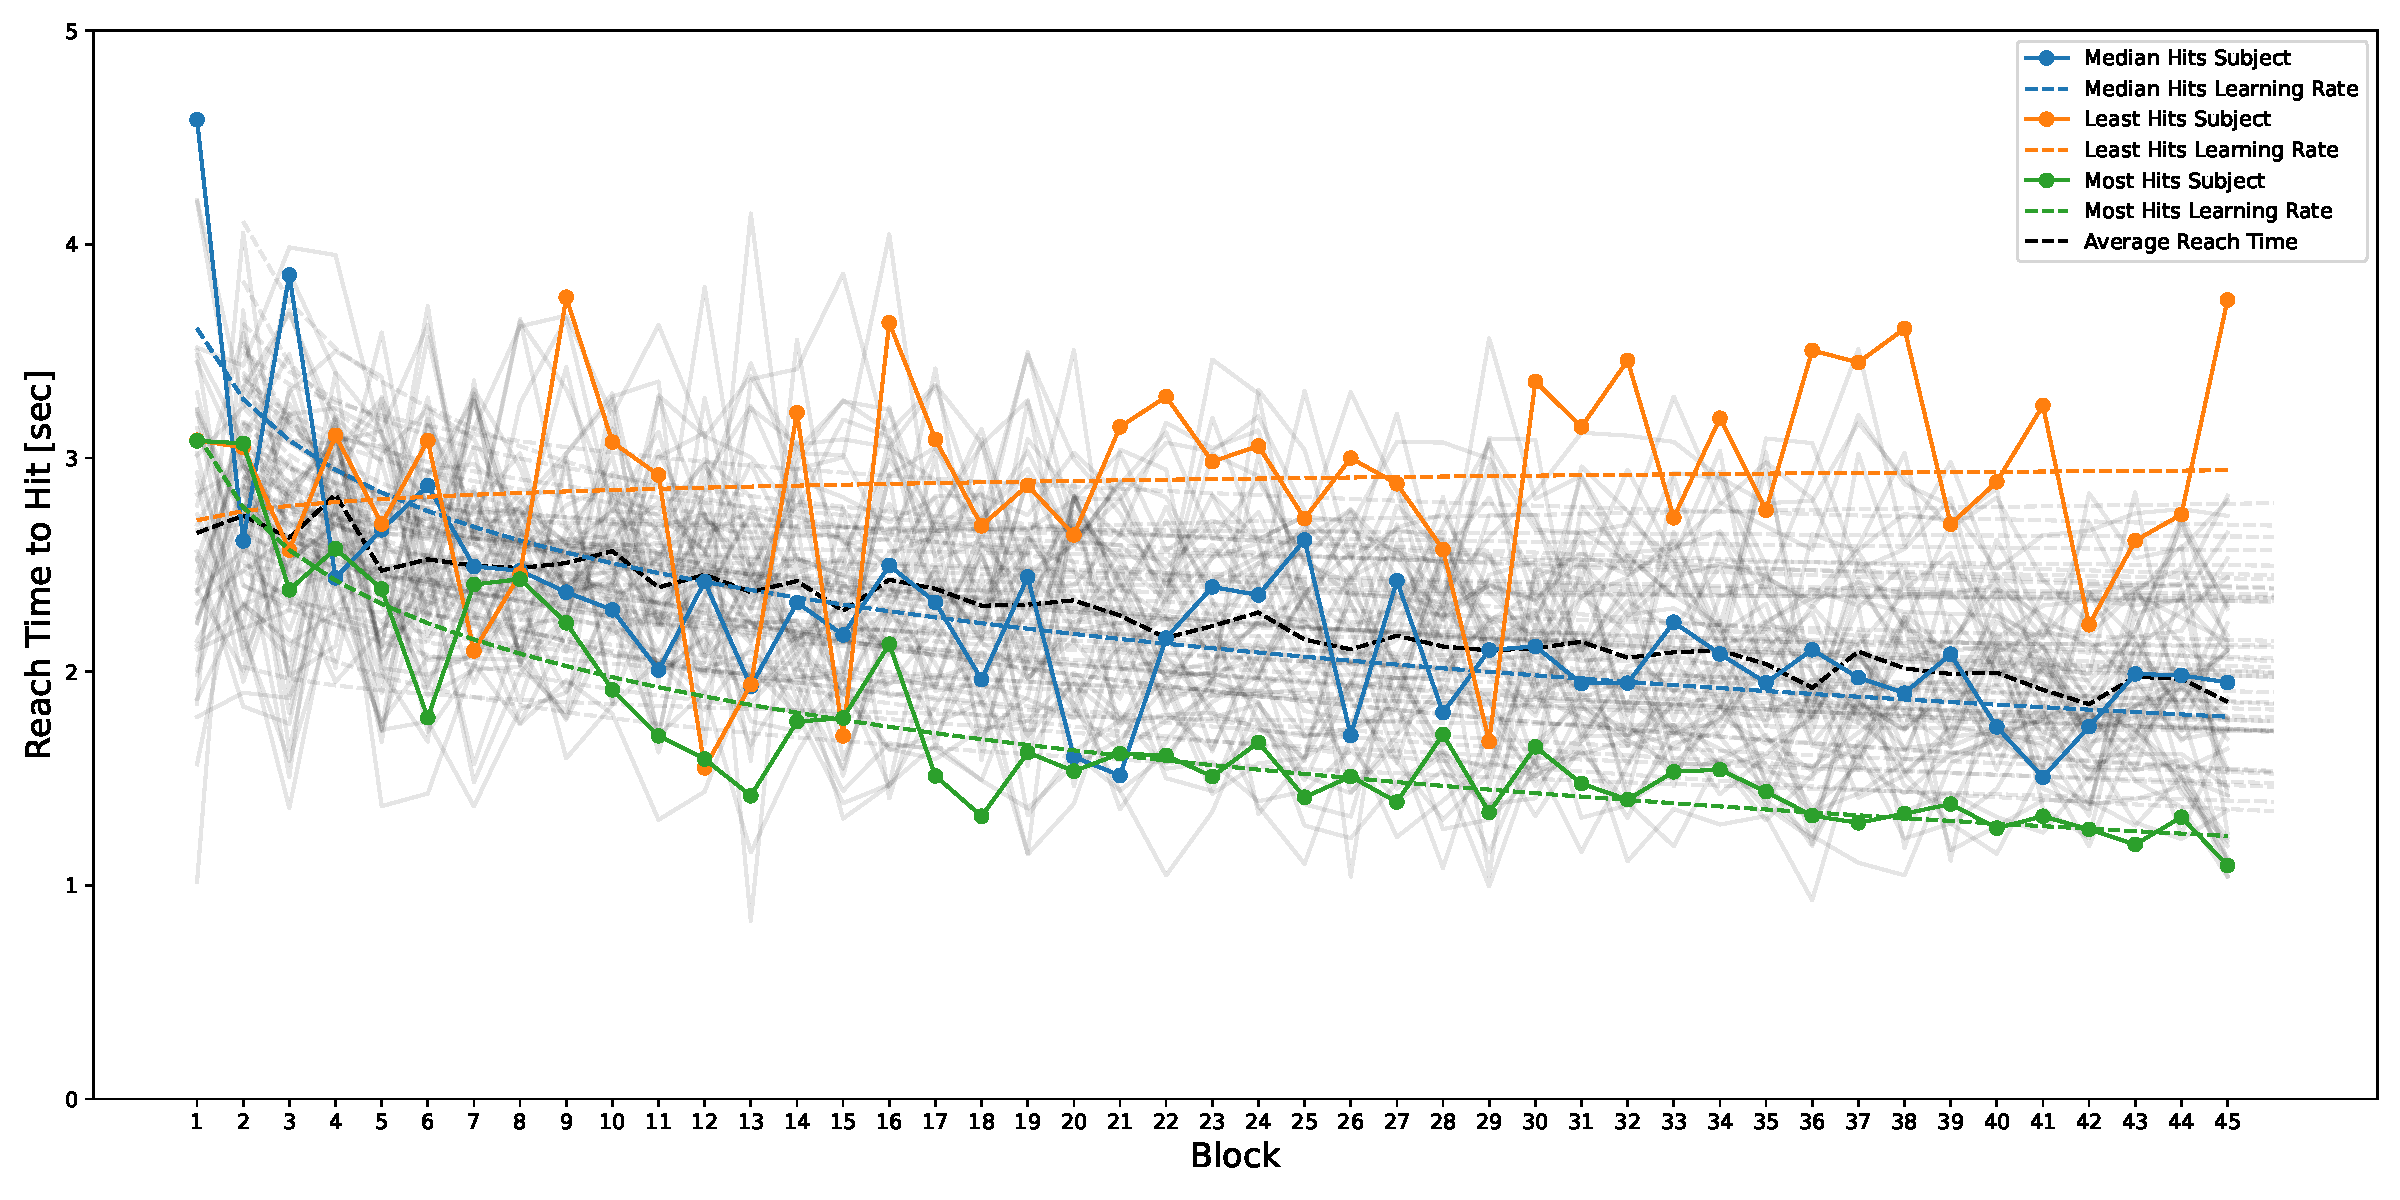
\includegraphics[width=1.0\textwidth]{basic_results/performance_over_blocks/reach_times_over_blocks.pdf}
    \caption[Reach time over trials]{Reach time over trials.}\label{fig:reach_times_over_blocks}
\end{figure}


\begin{figure}[H]%[tph]
    \centering
    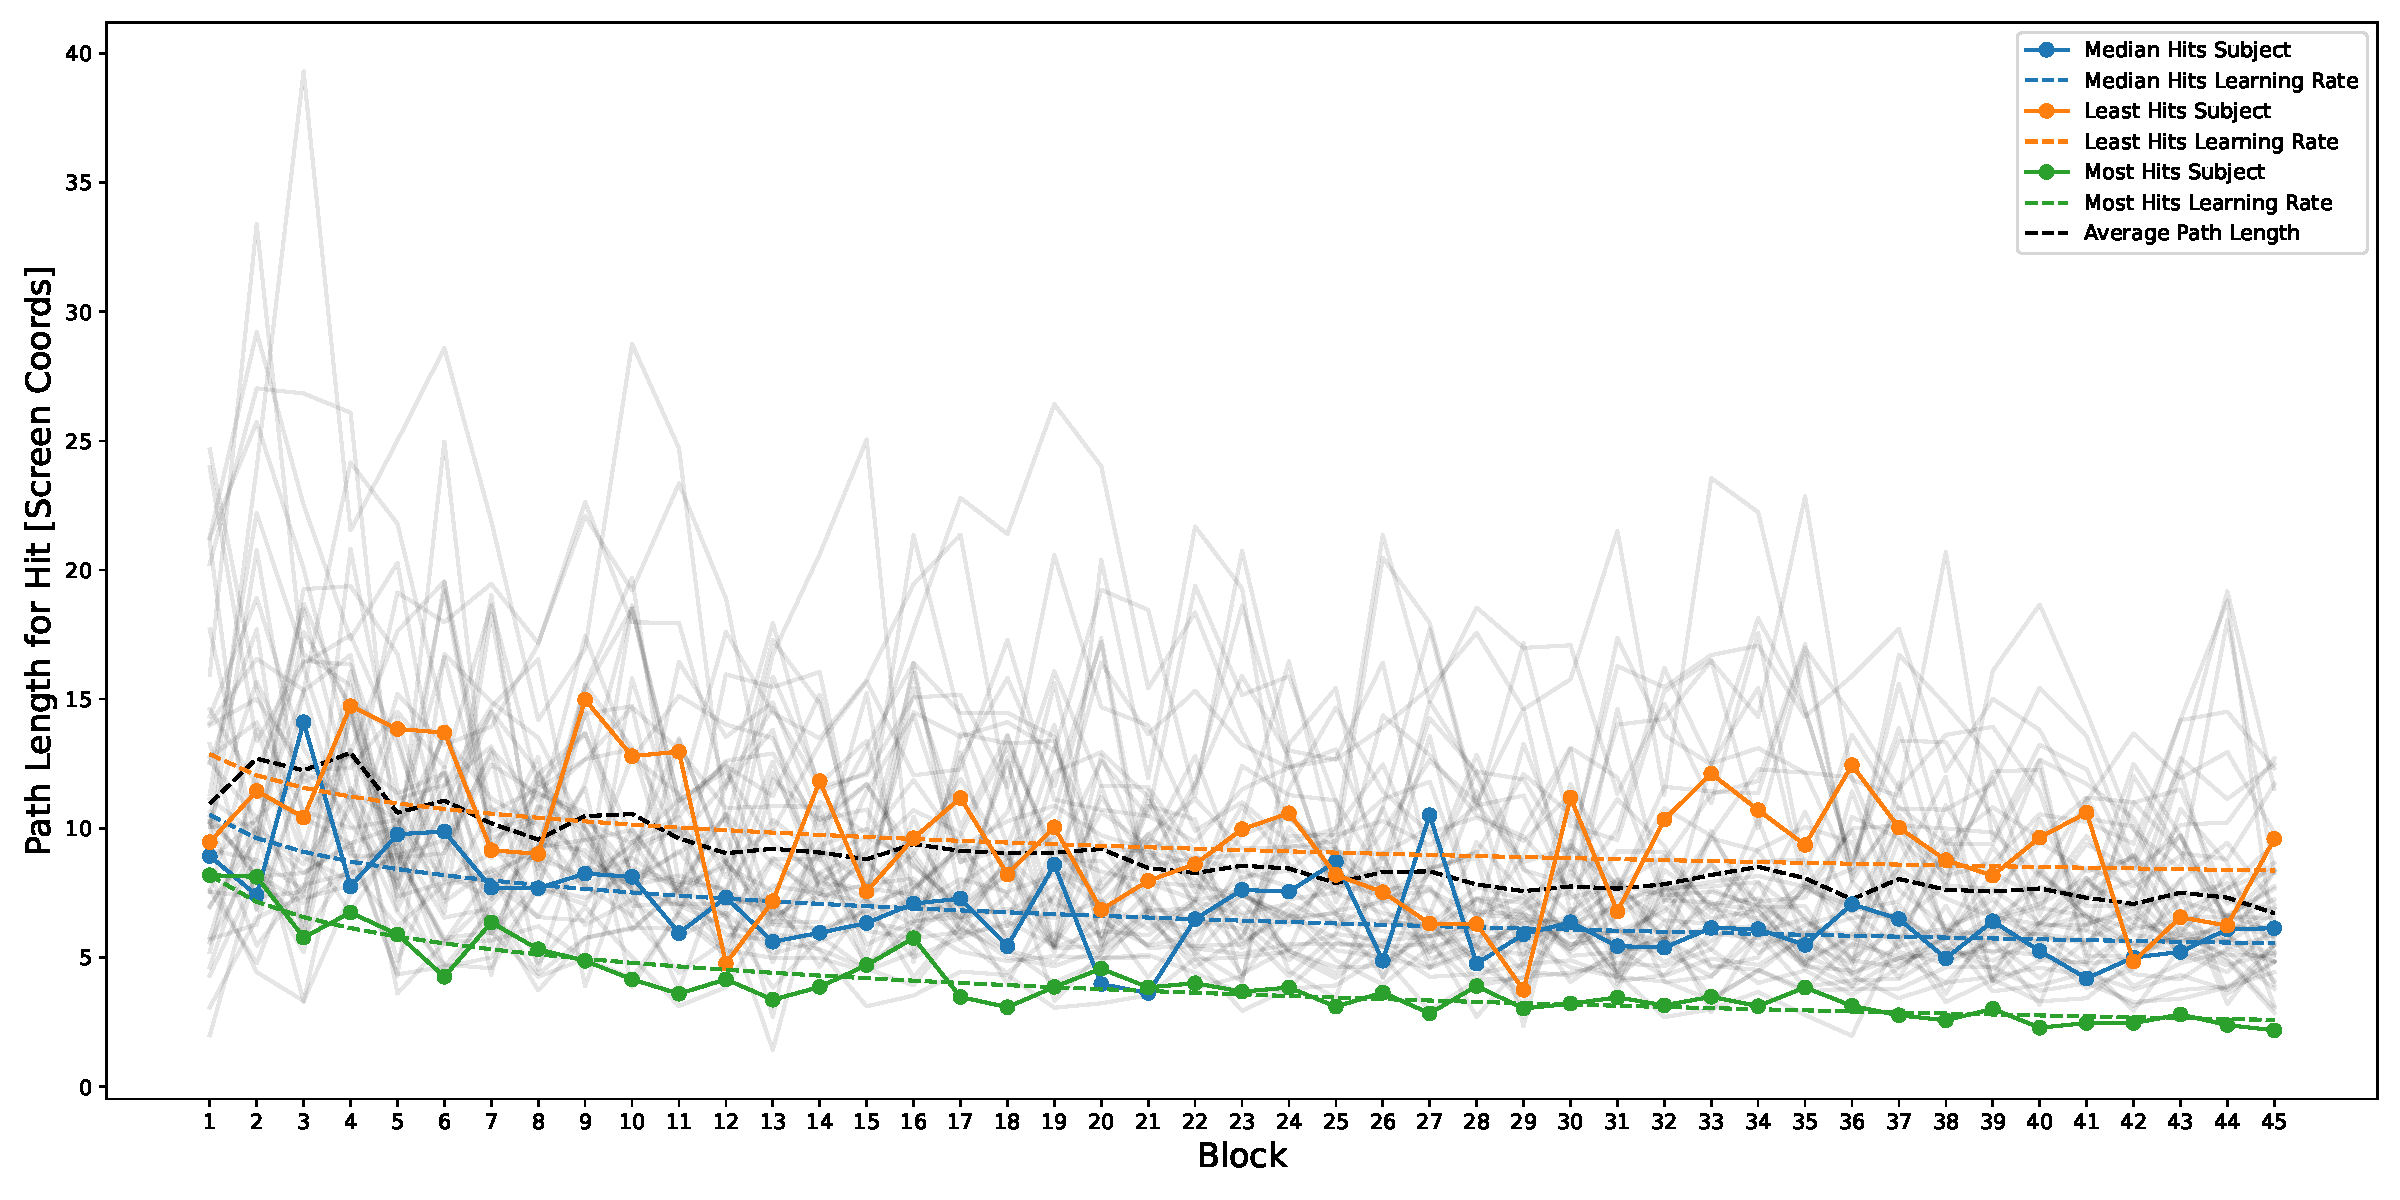
\includegraphics[width=1.0\textwidth]{basic_results/performance_over_blocks/path_length_over_blocks.pdf}
    \caption[Trajectory length over trials]{return np.sum (np.sqrt (np.sum (np.diff (a, axis=0)**2,axis=1)))}\label{fig:path_length_over_blocks}
\end{figure}


Path segments are defined as points where the sign of the trajectory's derivative changes, equivalent to ``zero crossings'' of the derivative. We filter low-velocity zero crossings and combine crossings that are close to one another. 

\begin{figure}[H]%[tph]
    \centering
    \includegraphics[width=1.0\textwidth]{basic_results/performance_over_blocks/path_segments_over_blocks.pdf}
    \caption[Trajectory segments over trials]{This connects to the idea of freezing degrees of freedom. We expect to see degrees of freedom in the task space, quantified by segments, to decrease over trials.}\label{fig:path_segments_over_blocks}
\end{figure}


\begin{figure}[H]%[tph]
    \centering
    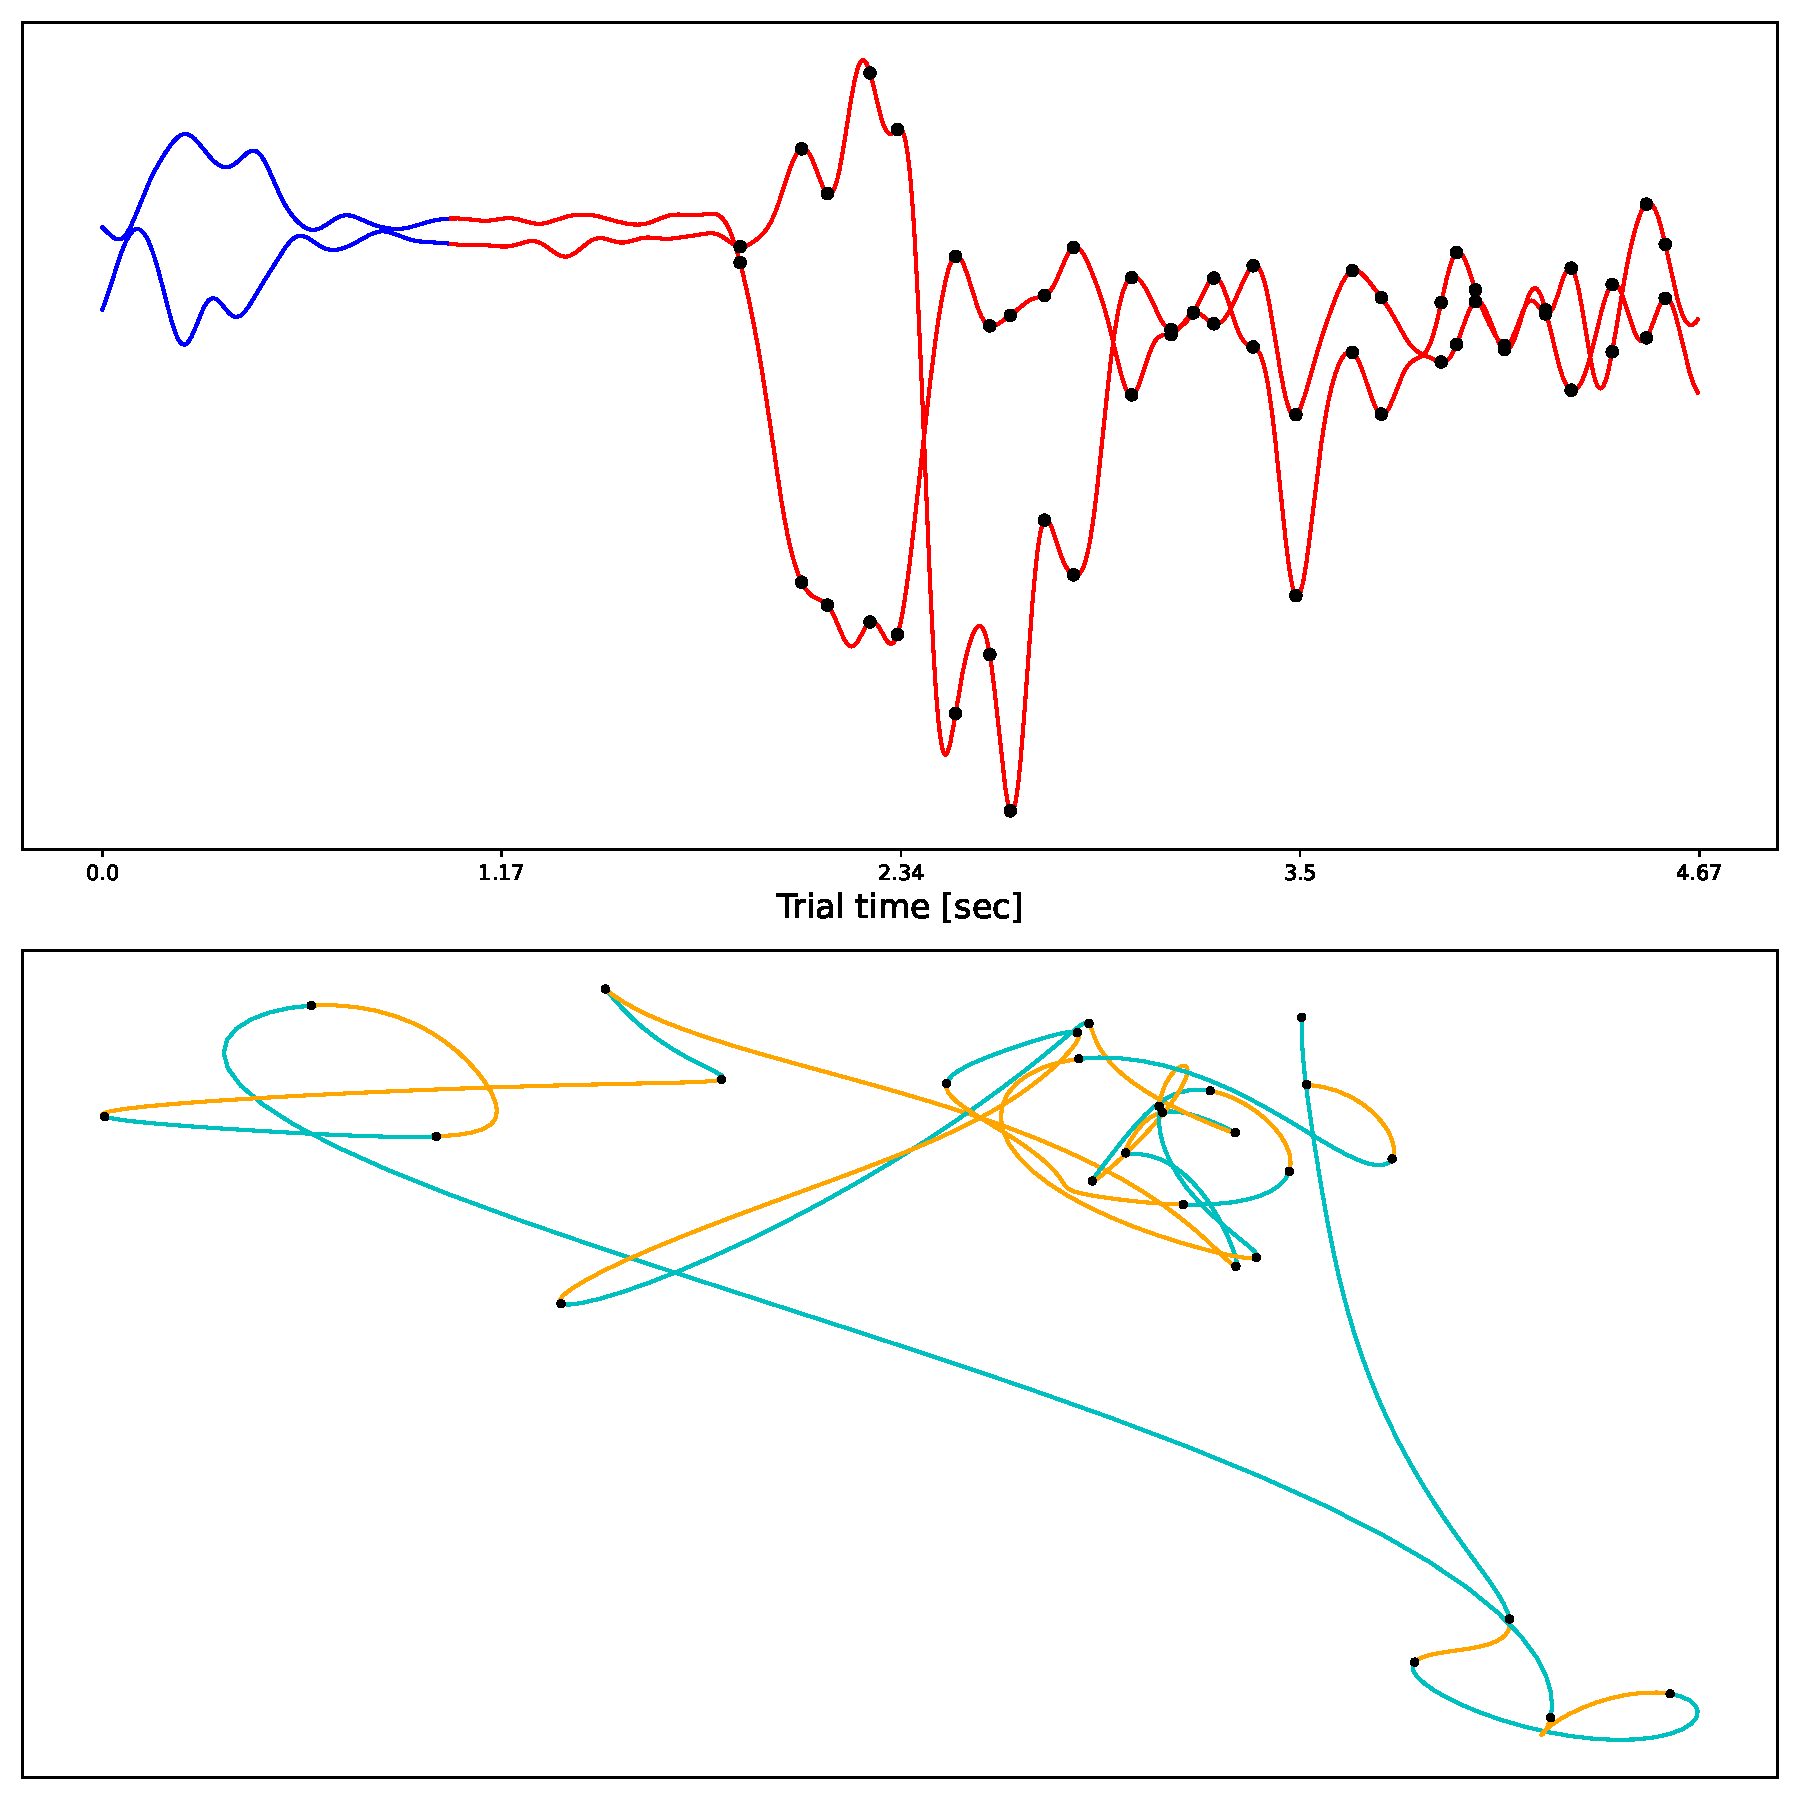
\includegraphics[width=1.0\textwidth]{basic_results/performance_over_blocks/example_path_segments.pdf}
    \caption[Example of a path segmented trial]{Example path segmentation. Path segments are defined as zero crossings of the trajectory's derivative. We then combine crossings that are near each other in time, and exclude crossings below the 10th percentile of the max velocity in order to remove short segments.}\label{fig:example_segments}
\end{figure}


\begin{table}[H]
    \begin{center}
        \caption[Statistics of performance regression]{Statistics of performance regression}\label{tab:performance_stats}
        \begin{tabular}{l | c}
            \hline
            $p$(Hit Learning Rate, Reward) & 0.177 \\
            $p$(Reach time Learning Rate, Reward) & 0.215 \\
            $p$(Path length Learning Rate, Reward) & 0.786 \\
            $p$(Segment Learning Rate, Reward) & 0.072 \\
            Adjusted R-squared & 0.058 \\
            Prob (F-statistic) & 0.170
        \end{tabular}
    \end{center}
  \end{table}
  
% mean_reward vs [hit_learning_rates, reach_time_learning_rates, path_length_learning_rates, segment_learning_rates]

% OLS Regression Results                            
% ==============================================================================
% Dep. Variable:                      y   R-squared:                       0.142
% Model:                            OLS   Adj. R-squared:                  0.058
% Method:                 Least Squares   F-statistic:                     1.693
% Date:                Wed, 14 Feb 2024   Prob (F-statistic):              0.170
% Time:                        10:31:57   Log-Likelihood:               -0.99915
% No. Observations:                  46   AIC:                             12.00
% Df Residuals:                      41   BIC:                             21.04
% Df Model:                           4                                         
% Covariance Type:            nonrobust                                         
% ==============================================================================
%                  coef    std err          t      P>|t|      [0.025      0.975]
% ------------------------------------------------------------------------------
% const          0.9233      0.114      8.083      0.000       0.693       1.054
% x1             0.0780      0.057      1.375      0.177      -0.037       0.193
% x2             0.7350      0.584      1.259      0.215      -0.444       1.914
% x3             0.0102      0.037      0.274      0.786      -0.065       0.085
% x4            -0.1088      0.059     -1.845      0.072      -0.228       0.010
% ==============================================================================
% Omnibus:                        4.990   Durbin-Watson:                   2.155
% Prob(Omnibus):                  0.083   Jarque-Bera (JB):                4.054
% Skew:                           0.477   Prob(JB):                        0.132
% Kurtosis:                       4.098   Cond. No.                         51.4
% ==============================================================================

\begin{itemize}
    \setlength\itemsep{0em}
    \item Reward correlates with hits, but noisily. Hits can happen with more or less reward. Reward is a more fine-grained signal of performance as it reflects the trajectory directly as opposed to the binary outcome of each movement. Higher reward implies more direct, straight-line trajectories to targets. Mean reward is based on active EMG samples.
    \item The learning rate for hits based on the logarithm fit to hit counts over blocks does not linearly correlate significantly with mean reward, indicating that the magnitude of the rate with which a subject accumulates hits over blocks does not necessarily lead to lower reward. This might be explained by the fact that some subjects start at high hit rate, meaning less learning is available to these subjects, meaning their learning rate is low despite their performance being high (reward being low). Note here that it may serve us well to look closely at subjects with high learning rates and high increases in performance over trials, as these subjects displayed the most learning, the largest spread in performance.
    \item Looking at the histograms of reward and hit counts per subject, we can justify using the mean reward per subject as a measure of performance as there are not any glaring outliers and the curve is approximately normal, while the hit count curve is skewed (\textbf{TODO?}: normality tests on these?)
    \item \textbf{TODO} make sure that I'm using active EMG to compute reward. Shouldn't change the statistics, but good to check.
    \item \textbf{TODO?} Put this histogram and the hits vs. reward plot first, then use reward everywhere instead of hits! 
\end{itemize}

Mean reward is defined over $K$ trials and samples or timepoints $T$ using the 2-norm of the distance between the cursor position $x$ and the target, or goal, position $g$ for a given timepoint $t$ and trial $k$:

\begin{align}
    r = \frac{1}{KT}\sum_k^K\sum_t^T{|| \vec{g_k} - \vec{x}_{t,k} ||^{-2}}.
    \label{eq:reward}
\end{align}

\begin{figure}[H]%[tph]
    \centering
    \includegraphics[width=1.0\textwidth]{basic_results/performance_over_blocks/hit_fraction_vs_reward.pdf}
    \caption[Hits versus reward]{Hit counts versus total reward.}\label{fig:hit_fraction_vs_reward}
\end{figure}

\begin{figure}
    \centering
    \begin{minipage}{0.49\textwidth}
        \includegraphics[width=0.9\textwidth]{basic_results/trial_reward/reward_histogram.pdf}
        \subcaption{}
    \end{minipage}
    \begin{minipage}{0.49\textwidth}
        \includegraphics[width=0.9\textwidth]{basic_results/trial_reward/hit_fraction_histogram.pdf}
      \subcaption{}
    \end{minipage}
    \caption[Hit and reward histograms]{Hits and rewards histograms over subjects}\label{fig:reward_histograms}
\end{figure}

% \begin{figure}[H]%[tph]
%     \centering
%     \includegraphics[width=1.0\textwidth]{basic_results/performance_over_blocks/mean_rewards_vs_learning_rate.pdf}
%     \caption[Reward versus learning rate]{No correlation between the rate of hit accumulation and total reward.}\label{fig:mean_rewards_vs_learning_rate}
% \end{figure}


\subsection{Hits over Targets}

\begin{itemize}
    \setlength\itemsep{0em}
    \item We find a significant difference in the mean number of hits between the directly rightward target, Target 1, and the leftward targets 6, 7, and 8. I would have to speculate on why this bias appears on average. It's probably best not to speculate, and just explain what this implies: that for some reason it's more likely to create a decoder which aligns with subject's more common movements in a leftward direction than a rightward one. Probably worth discussing here that next time, we need to think more carefully about the subject's inherent EMG manifold before mapping. This is kind of a bootstrapping problem-- we didn't know we would have this problem before we tried it out. Next time, I would more deeply explore the subject's EMG manifold and relate that to the task directly, by simulating their task-space EMG projection more fully, creating a decoder extraction pipeline that explicitly balanced activity between targets. \Cref{fig:hits_over_targets}
    \item This is also true for Target 4, straight up. I think this is due to how the decoder was made, by subtracting pairs of NMF modes. This, I think, means that you're less likely to get ``pure'' up and right. But this isn't true for left and down, the ``negative'' directions. I'm not sure why this is.
\end{itemize}

\begin{figure}[H]%[tph]
    \centering
    \begin{minipage}{1.0\textwidth}
        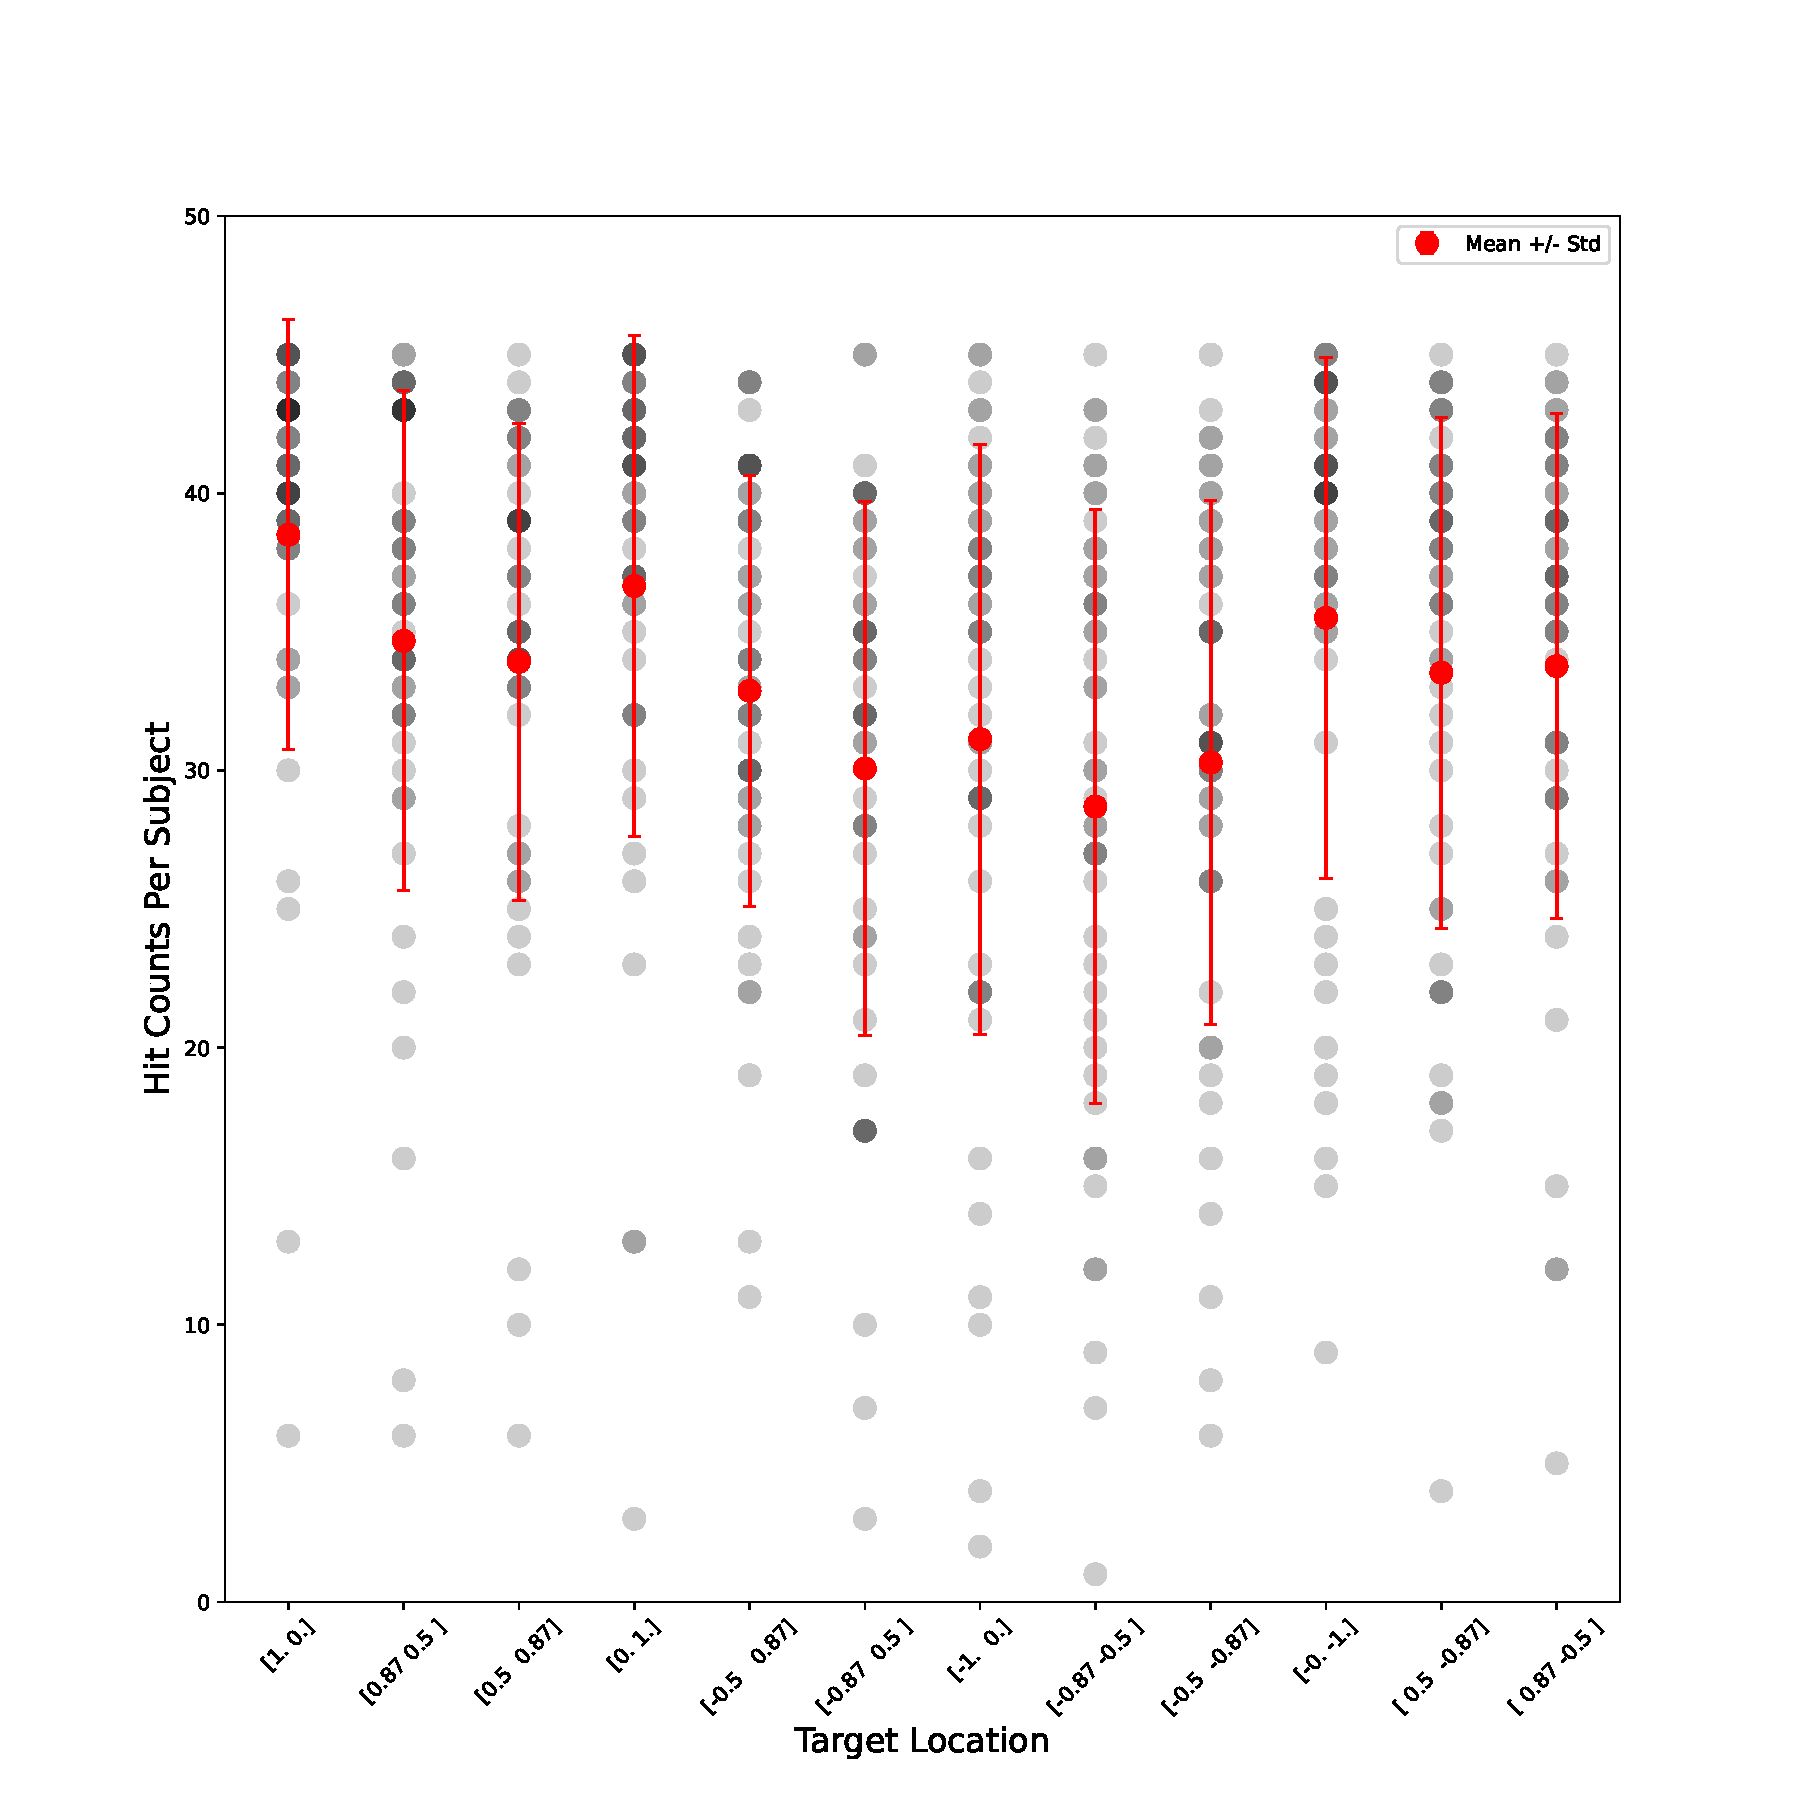
\includegraphics[width=1.0\textwidth]{basic_results/decoder_vs_performance/hits_over_targets.pdf}
        \subcaption{}
    \end{minipage}\\%
    \begin{minipage}{0.49\textwidth}
        \includegraphics[width=1.0\textwidth]{basic_results/decoder_vs_performance/target_means.pdf}
      \subcaption{}
    \end{minipage}
    \begin{minipage}{0.49\textwidth}
        \includegraphics[width=1.0\textwidth]{basic_results/decoder_vs_performance/target_hit_pvalues.pdf}
      \subcaption{}
    \end{minipage}
    \caption[Hits over Targets across subjects]{Hit count means per target. Significance matrix comparing hit counts over individual targets to assess bias in target directions across subjects.}\label{fig:hits_over_targets}
\end{figure}





\section{Do Subject Attributes Predict Performance?}

\begin{itemize}
    \setlength\itemsep{0em}
    \item Look at self-reported form response data to explore whether there are obvious confounds based on subject metadata
    \begin{itemize}
        \item Arm size --- measured the circumference of the arm 5cm below the tip of the elbow --- weak correlation! This implies that those with larger arms perform better on the task. We speculate that this may be due to subjects with larger arms allowing electrodes to cover more motor units, thus allowing for greater decorrelation between EMG channels. We explore this more deeply in later chapters using a metric we term ``subspace confinement''.
        \item Time order of the subject out of the cohort of 46 subjects --- no correlation
        \item Time of day data collection began --- no correlation
        \item Hours of sleep reported --- no correlation
        \item Sex --- significant difference in mean! This, we suspect, is explained by arm size
        \item Sportsperson --- none 
        \item handedness --- none, though few left handed subjects
        \item caffeine consumption day of the experiment grouped into high and low --- none 
        \item self-described as dexterous or engaging in tasks considered dexterous --- none
        \item In all, these categorical results are promising as they signify that our task presents a novel challenge for subjects, in the sense that it is dissimilar from other activities and thus does not provide an advantage.
        \item The only advantage we found was due to arm size.
        \item \textbf{TODO} --- statistics for mean comparisons in \Cref{fig:compare_subject_groups}
    \end{itemize}
\end{itemize}


\begin{figure}[H]%[tph]
    \centering
    \includegraphics[width=1.0\textwidth]{basic_results/form_response/arm_vs_reward.pdf}
    \caption[Arm versus reward]{}\label{fig:arm_vs_reward}
\end{figure}

\begin{figure}[H]%[tph]
    \centering
    \includegraphics[width=1.0\textwidth]{basic_results/form_response/days_vs_reward.pdf}
    \caption[Experiment day versus reward]{}\label{fig:days_vs_reward}
\end{figure}

\begin{figure}[H]%[tph]
    \centering
    \includegraphics[width=1.0\textwidth]{basic_results/form_response/hour_of_day_vs_reward.pdf}
    \caption[Hour of day versus reward]{}\label{fig:hour_of_day_vs_reward}
\end{figure}

\begin{figure}[H]%[tph]
    \centering
    \includegraphics[width=1.0\textwidth]{basic_results/form_response/sleep_vs_reward.pdf}
    \caption[Hours of sleep vs reward]{}\label{fig:sleep_vs_reward}
\end{figure}

\begin{figure}[H]%[tph]
    \centering
    \includegraphics[width=1.0\textwidth]{basic_results/form_response/compare_subject_groups.pdf}
    \caption[Subject group comparisons]{}\label{fig:compare_subject_groups}
\end{figure}



\section{Does the Decoder Predict Performance?}

\begin{itemize}
    \setlength\itemsep{0em}
    \item How do decoders act on EMG data? We took uniformly random EMG and projected it onto all subject decoders, and show that only one decoder resulted in data that rejected normality. \Cref{fig:decoder_normality}. The decoders act on EMG data by effectively gaussian blurring the data centered on the center of the task space.
    \item Do the directions of the decoder correlate with performance? See example decoders in \Cref{fig:decoder_arrows}. We found no significant correlation in the alignment, measure by cosine similarity, of the two decoder axes, and mean reward. This implies the decoder axes orthogonality neither handicaps nor gives an advantage to subjects, sww \Cref{fig:decoder_cosine_vs_reward}
    \item \textbf{TODO} Plot the mean of all subjects decoder arrows, which may help to explain the bias towards the left hand side of the screen? However, this is a weird average to take since the order of EMG channels will differ. I would need to do this using some kind of density plot, overlaying each subject's deocder arrows in 2D. Probably more trouble than it's worth.
\end{itemize}

    Hypothesis: yes, decoder directions which happen to be oriented towards targets will make the learning problem easier, and thus correlate positively with performance.

If the decoder directions are more/less aligned to the target directions, do subjects explore less/more? Is exploration (e.g. EMG variance) higher in subjects with misaligned decoders?
    Hypothesis: exploration will be lower in subjects with target-aligned decoders. Subjects make fewer incorrect movements, and thus are induced to explore less.

\begin{figure}[H]%[tph]
    \centering
    \includegraphics[width=1.0\textwidth]{basic_results/decoder_vs_performance/decoder_arrows.pdf}
    \caption[Example decoder directions in 2D.]{Example decoders directions in 2D.}\label{fig:decoder_arrows}
\end{figure}

\begin{figure}[H]%[tph]
    \centering
    \includegraphics[width=1.0\textwidth]{basic_results/decoder_vs_performance/decoder_normality_test.pdf}
    \caption[Decoder normality testing]{Testing the effect of the decoder on uniform data.}\label{fig:decoder_normality}
\end{figure}

\begin{figure}[H]%[tph]
    \centering
    \includegraphics[width=1.0\textwidth]{basic_results/decoder_vs_performance/decoder_cosine_vs_reward.pdf}
    \caption[Decoder axis similarity versus reward]{Decoder cosine similarity. EMG-to-force decoders are computed using a calibration dataset collected before the ``center hold, reach out'' task. 4 ``modes'' of EMG activity are extracted from the dataset using non-negative matrix factorization. These 4 modes are then subtracted in pairs to yield the two 64-dimensional EMG-to-force mappings, shown in \{+@fig:low\_variance\_PCs\}. The left plot shows the cosine similarity of the $x$ and $y$ EMG-to-force decoders. A cosine similarity of 1 means the two vectors are parallel, producing identical forces (in the respective directions) for the same EMG activity ($F_x = F_y$). A cosine similarity of -1 means the vectors are antiparallel, producing equal but opposite forces in the two directions ($F_x = -F_y$). A cosine similarity of 0 means the decoder directions are orthogonal; e.g.producing a force in the $x$ direction with a certain EMG activity produces no force in the $y$ direction. Plotted across subjects, we see a range of decoder similarities, providing a variety of task contingencies. The rightmost plot asks whether cosine similarity is predictive of task success, in terms of the numbers of ``Hits''. We find no significant correlation, implying that the decoder cosine similarity, in the range we tested, does not predict task success. Task success, therefore, likely relies on an alternative task variable.}\label{fig:decoder_cosine_vs_reward}
\end{figure}

% \begin{figure}[H]%[tph]
%     \centering
%     \includegraphics[width=0.8\textwidth]{basic_results/decoder_vs_performance/mean_decoder.pdf}
%     \caption[Decoder normality testing]{Average decoder over subjects}\label{fig:mean_decoder}
% \end{figure}



\section{Does Task Space Variance Decrease over Trials?}

\begin{itemize}
    \setlength\itemsep{0em}
    \item \textbf{TODO} This section is confused and needs rethinking or cutting. The point is to show that trajectory variance decreases over time. This isn't a very interesting point to make, as it's clear that this is the case from the earlier performance plots. Should we really only be looking at the $y$ coordinate since the $x$ coordinate has to vary in order to hit the target?
    \item Looking at the example trajectories in \Cref{fig:mean_trajectories}, with means shown in color are averaged over trajectories normalized in time such that they have identical length. This is achieved by interpolating shorter trajectories. We can see that higher performing subjects have less erratic movements, and seem to use the dominant directions of their underlying EMG manifold, projected onto the task plane, to their advantage.
    \item \Cref{fig:rotated_trajectories} shows how trajectories are rotated for comparison. The blue trajectories have been rotated such that every goal state or pseudo-target is Target 1, purely rightward. \textbf{TODO} plot the targets.
    \item \Cref{fig:trajectory_variance} shows that trajectory variance in the $x$ and $y$ directions tends to decrease exponentially, plotting the log as subject variance is right-tailed. 
    \item \textbf{TODO} should we show the right-tailed data here too? Should we fit this exponential, in order to say ``across subjects on average trajectory variance decreases'' We could try to relate this to performance, maybe showing correlation between early and late variance? There might be a point made here about exploration in the task space? The original idea here was to explore the task space statistics more fully before getting into the full EMG space. The decoder discussion about normality allows us to say that the decoder is a projection onto a 2d plane, but going from 64 to 2 dimensions also has this concentrating action, so the task space statistics are interesting on their own as well. This is still unrealized here. Unclear what the story can or should be.
\end{itemize}



\begin{figure}[H]%[tph]
    \centering
    \includegraphics[height=0.9\textheight]{basic_results/mean_trajectories/mean_trajectories.pdf}
    \caption[Mean trajectories]{??}\label{fig:mean_trajectories}
\end{figure}


\begin{figure}[H]%[tph]
    \centering
    \includegraphics[width=\textwidth]{basic_results/trajectory_variance/rotated_trajectories.pdf}
    \caption[Rotating trajectories]{??}\label{fig:rotated_trajectories}
\end{figure}


\begin{figure}[H]%[tph]
    \centering
    \includegraphics[width=1.0\textwidth]{basic_results/trajectory_variance/trajectory_variance_over_blocks.pdf}
    \caption[Trajectory variance over blocks]{Plotting the log as variance tends to decrease exponentially}\label{fig:trajectory_variance}
\end{figure}


% cut this as it's shit
% \begin{figure}[H]%[tph]
%     \centering
%     \begin{minipage}{0.9\textwidth}
%         \includegraphics[width=\textwidth]{basic_results/trajectory_variance/trajectory_r_squared_fit.pdf}
%         \subcaption{}
%     \end{minipage}\\%
%     \begin{minipage}{0.9\textwidth}
%         \includegraphics[width=0.8\textwidth]{basic_results/trajectory_variance/trajectory_variance_slope.pdf}
%       \subcaption{}
%     \end{minipage}
%     \caption[Trajectory variance statistics]{Trajectory variance statistics}\label{fig:trajectory_variance_fits}
% \end{figure}




\cleardoublepage\printendnotes%
\ifSubfilesClassLoaded{%
    \newpage%
    \bibliography{../bib/bibliography}%
}{}%
\end{document}